\documentclass[a4paper, 12pt]{article}
\usepackage[utf8]{inputenc}
\usepackage[T1]{fontenc}
\usepackage{graphicx}
\usepackage{amsmath}
\usepackage{listings}
\usepackage{xcolor}
\usepackage{hyperref}
\usepackage{caption}
\usepackage{subcaption}
\usepackage{booktabs}
\usepackage{array}

\usepackage[margin=0.8in]{geometry} % Compact margins
\usepackage{setspace} % line spacing control
\usepackage{parskip}  % No paragraph indentation
\usepackage{ragged2e} % Better left alignment

% Code listing style
\lstset{
    language=Python,
    basicstyle=\ttfamily\small,
    keywordstyle=\color{blue},
    commentstyle=\color{green},
    stringstyle=\color{red},
    frame=single,
    breaklines=true,
    postbreak=\mbox{\textcolor{red}{$\hookrightarrow$}\space},
}

% Hyperref setup
\hypersetup{
    colorlinks=true,
    linkcolor=blue,
    filecolor=magenta,      
    urlcolor=cyan,
    pdftitle={Business-IT Alignment Dynamics},
    pdfpagemode=FullScreen,
}

\title{Business-IT Alignment Dynamics: A Chaotic Systems Approach}
\author{Alessandro Aquilini}
\date{\today}

\begin{document}
\pagestyle{empty}
\setstretch{1.1} % 1.1x line spacing
\raggedright     % clean left alignmen

\maketitle

\begin{abstract}
	This report investigates the dynamics of Business-IT alignment through a discrete-time chaotic model. The proposed equation captures how environmental pressures, IT department efficacy, and organizational adaptability interact to create alignment or misalignment patterns. Through numerical simulations and bifurcation analysis, we identify conditions leading to stable alignment, oscillations, and chaotic behavior.
\end{abstract}

\tableofcontents

\section{Introduction}
\subsection{Objective}
The project aims to model Business-IT alignment dynamics using a discrete-time equation that exhibits chaotic behavior under certain parameter conditions. The primary goals are:

\begin{itemize}
	\item Develop a mathematical model of alignment evolution
	\item Implement interactive simulations in Python
	\item Analyze stability and chaotic regimes
	\item Provide visual tools for parameter exploration
\end{itemize}

\subsection{Key Findings}
\begin{itemize}
	\item The system shows three characteristic behaviors: convergence, oscillations, and chaos
	\item IT department efficacy ($a$) and system rigidity ($h$) have non-linear effects
	\item Organizational flexibility ($s$) determines adaptation sharpness
	\item Bifurcation diagrams reveal parameter regions of chaotic behavior
\end{itemize}

\section{Model Description}
\subsection{Core Equation}
The alignment dynamics are governed by:

\begin{equation}
	x_{t + 1} = x_t + A(x_t) - B(x_t)C(x_t)
\end{equation}

Where:
\begin{itemize}
	\item $x_t$: Percentage of dissatisfied users (misalignment proxy)
	\item $A(x_t)$: Environmental pressure effect
	\item $B(x_t)$: IT department efficacy
	\item $C(x_t)$: Organizational adaptability
\end{itemize}

\subsection{Component Functions}
\begin{align}
	A(x_t) & = d(1 - x_t)                                                                     \\
	B(x_t) & = \frac{a x_t (1 - x_t)^g}{1 + a h x_t}                                          \\
	C(x_t) & = \frac{1}{1 + z^s} \quad \text{where} \quad z = \frac{r (1 - x_t)}{x_t (1 - r)}
\end{align}

\subsection{Parameter Definitions}
\begin{table}[h]
	\centering
	\caption{Model Parameters and Ranges}
	\begin{tabular}{llll}
		\toprule
		\textbf{Parameter} & \textbf{Description}       & \textbf{Range} & \textbf{Default} \\
		\midrule
		$x_0$              & Initial misalignment       & [0.01, 0.99]   & 0.3              \\
		$d$                & Environmental dynamicity   & [0.01, 5]      & 0.5              \\
		$a$                & IT department efficacy     & [0.1, 10]      & 2                \\
		$h$                & IT system rigidity         & [0.1, 5]       & 1                \\
		$g$                & IT investment propensity   & [0.1, 5]       & 1                \\
		$r$                & Action threshold           & [0.01, 0.99]   & 0.3              \\
		$s$                & Organizational flexibility & [1, 10]        & 3                \\
		\bottomrule
	\end{tabular}
\end{table}

\subsection{Interpretation}
Let's take a deeper look at our equation:

\begin{equation}
	x_{t + 1} = x_t + \underbrace{A(x_t)}_{\text{Environmental Pressure}} - \underbrace{B(x_t)C(x_t)}_{\text{Recovery Mechanism}}
\end{equation}

\begin{description}
	\item[$x_t$ \textendash\ Alignment] Measures the percentage of dissatisfied users at time $t$:
		\begin{itemize}
			\item $0 \rightarrow$ Complete satisfaction (perfect alignment)
			\item $1 \rightarrow$ Utter dissatisfaction (total misalignment)
		\end{itemize}

	\item[$A(x_t)$ \textendash\ Environmental Pressure:] Increases misalignment due to external factors, representing how competitive environments and technological changes increase dissatisfaction.

	\item[$B(x_t) \cdot C(x_t)$ \textendash\ Recovery Mechanism:] Reduces misalignment through:
		\begin{itemize}
			\item $B(x_t)$: IT department's effectiveness.
			\item $C(x_t)$: Organization's adaptability.
		\end{itemize}
\end{description}

\subsection{Parameter Analysis}
Full interactive simulation available at: \url{https://www.desmos.com/calculator/n55bwehjlp}

\subsubsection{Environmental Pressure Function}
\begin{equation}
	A(x_t) = d(1 - x_t)
\end{equation}

Forms a line passing through $(1, 0)$ with slope $-d$.
\begin{itemize}
	\item \textbf{$d$ (dynamicity)}: Fast changing industries (e.g., a tech startup) have a competition/innovation that rapidly renders old IT systems obsolete.
	\item \textbf{$1 - x_t$}: As misalignment grows, environmental pressure has less "room" to worsen things.
\end{itemize}

\begin{figure}[h]
	\centering
	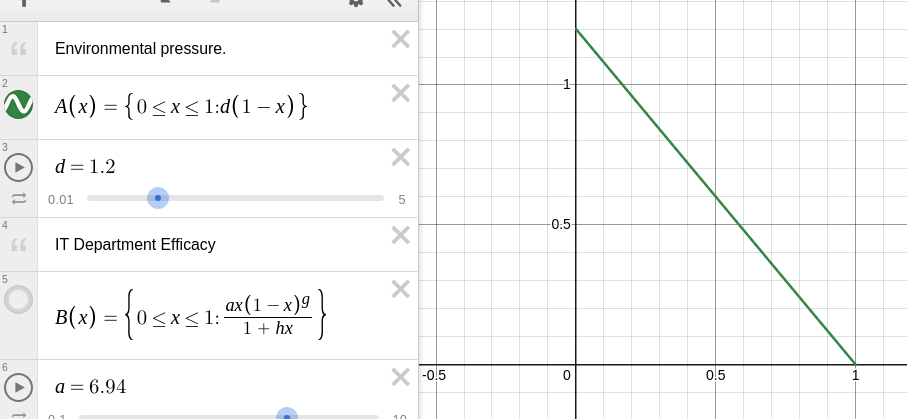
\includegraphics[width=0.8\textwidth]{../images/A(x)-desmos.png}
	\caption{Environmental pressure function for varying $d$ values}
\end{figure}

\subsubsection{IT Department Efficacy}
\begin{equation}
	B(x_t) = \frac{a x_t (1 - x_t)^g}{1 + a h x_t}
\end{equation}

This looks like a function that peaks at some $x_a$ and then tapers off.

\begin{itemize}
	\item \textbf{a (IT efficacy)}: an higher a can more effectively reduce misalignment.
	\item \textbf{x (current misalignment)}: the more misalignment exists, the more opportunity/pressure there is for IT to act.
	\item \textbf{$(1 - x_t)^g$ (Diminishing Returns)}: as satisfaction improves, the IT department's impact diminishes.
	      \begin{itemize}
		      \item I haven't understood g.
	      \end{itemize}
	\item \textbf{$1 + ahx_t$ (Saturation)}: even if IT is highly capable (a >> 1), inflexible systems (h >> 1) limit its efficacy.
\end{itemize}

\begin{figure}[h]
	\centering
	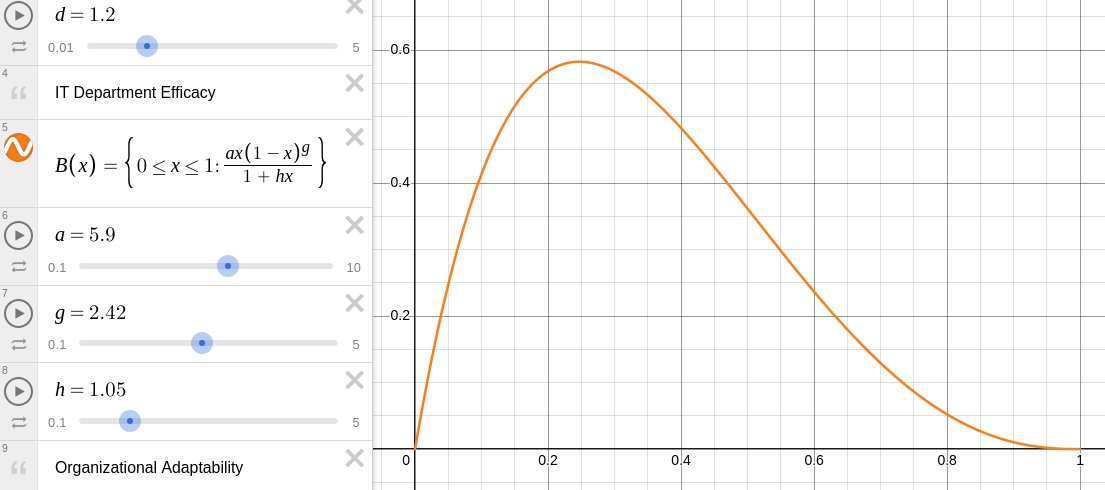
\includegraphics[width=0.8\textwidth]{../images/B(x)-desmos.png}
	\caption{IT efficacy function showing the effect of parameters $a$, $h$, and $g$}
\end{figure}

\subsubsection{Organizational Adaptability}
\begin{equation}
	C(x_t) = \frac{1}{1 + z^s} \quad \text{where} \quad z = \frac{r (1 - x_t)}{x_t (1 - r)}
\end{equation}

This is a \textbf{sigmoid} function in disguise. Sigmoids are exploited for modeling "threshold behaviors".

\begin{itemize}
	\item \textbf{r (activation threshold)}: below r, the organization resists to change ($C(x) \rightarrow 0$). But when misalignment crosses a certain threshold adaptability kicks in.
	\item \textbf{s (flexibility)}: higher s make the sigmoid steeper (sharper transition from resistance to adaptation).
\end{itemize}

\begin{figure}[h]
	\centering
	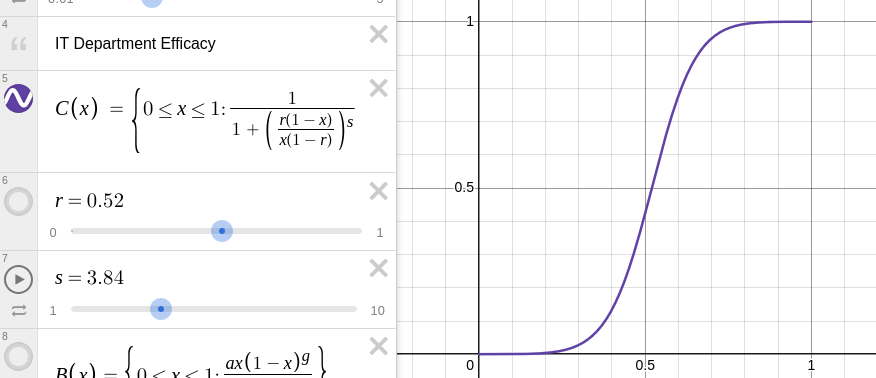
\includegraphics[width=0.8\textwidth]{../images/C(x)-desmos.png}
	\caption{Organizational adaptability function demonstrating threshold behavior}
\end{figure}


\section{Implementation}
\subsection{Technological Stack}
\begin{itemize}
	\item Python 3.x with NumPy/SciPy for numerical computation
	\item Matplotlib for visualization
	\item Jupyter Notebook for interactive exploration
	\item ipywidgets for parameter sliders
\end{itemize}

\subsection{Key Algorithms}
The implementation features:
\begin{itemize}
	\item Discrete-time simulation of the alignment equation
	\item Adaptive clipping to maintain $x_t \in [0,1]$
	\item Stability detection through final value analysis
	\item Bifurcation diagram generation
\end{itemize}

\begin{lstlisting}[caption=Core Simulation Code]
def simulate(x0, d, a, h, g, r, s, steps=50):
    x = np.zeros(steps)
    x[0] = x0
    for t in range(steps - 1):
        x[t + 1] = x[t] + delta(x[t], d, a, h, g, r, s)
        x[t + 1] = np.clip(x[t + 1], 0, 1)
    return x
\end{lstlisting}

\section{Results}
\subsection{Time Evolution}
\begin{figure}[h]
	\centering
	% \includegraphics[width=0.8\textwidth]{}
	\caption{Typical system evolution showing convergence to partial alignment}
\end{figure}

The simulation identifies three terminal states:
\begin{itemize}
	\item Aligned ($x < 0.1$)
	\item Partially Aligned ($0.1 \leq x \leq 0.9$)
	\item Misaligned ($x > 0.9$)
\end{itemize}

\subsection{Phase Portrait}
\begin{figure}[h]
	\centering
	% \includegraphics[width=0.8\textwidth]{}
	\caption{Phase portrait showing fixed points and flow directions}
\end{figure}

Key observations:
\begin{itemize}
	\item Stable fixed points occur where $dx/dt = 0$ with negative slope
	\item Color intensity shows rate of change magnitude
	\item Arrows indicate direction of alignment evolution
\end{itemize}

\subsection{Parameter Analysis}
\begin{figure}[h]
	\centering
	% \includegraphics[width=0.8\textwidth]{}
	\caption{Alignment as function of IT efficacy ($a$) and rigidity ($h$)}
\end{figure}

The contour plot reveals:
\begin{itemize}
	\item High efficacy + low rigidity → Best alignment
	\item Low efficacy + high rigidity → Worst alignment
	\item Non-linear interaction between parameters
\end{itemize}

\subsection{Chaotic Behavior}
\begin{figure}[h]
	\centering
	% \includegraphics[width=0.8\textwidth]{}
	\caption{Bifurcation diagram showing transition to chaos}
\end{figure}

Chaos appears when:
\begin{itemize}
	\item $g \approx 1.7$ with large $a$
	\item Certain combinations of $d$ and $h$
	\item The system undergoes period-doubling cascades
\end{itemize}

\section{Original Contributions}
\subsection{Key Innovations}
\begin{itemize}
	\item Developed a novel discrete-time model for Business-IT alignment
	\item Implemented interactive exploration tools
	\item Identified chaotic regimes in organizational dynamics
	\item Created comprehensive visualization methods
\end{itemize}

\subsection{Technical Challenges}
\begin{itemize}
	\item Numerical stability with extreme parameter values
	\item Efficient bifurcation diagram generation
	\item Interactive widget synchronization
	\item Chaotic regime detection
\end{itemize}

\section{Conclusion}
The project successfully:
\begin{itemize}
	\item Demonstrated chaotic behavior in Business-IT alignment
	\item Provided tools for parameter sensitivity analysis
	\item Identified conditions leading to stable alignment
	\item Offered visual methods for system state classification
\end{itemize}

Future work could explore:
\begin{itemize}
	\item Continuous-time versions of the model
	\item Multi-dimensional extensions
	\item Machine learning for parameter estimation
	\item Empirical validation with real-world data
\end{itemize}

\section*{References}
\begin{thebibliography}{9}
	\bibitem{chaos}
	Strogatz, S. H. (2018). \textit{Nonlinear dynamics and chaos: with applications to physics, biology, chemistry, and engineering}. CRC Press.

	\bibitem{italign}
	Luftman, J. (2003). \textit{Assessing IT/business alignment}. Information Systems Management, 20(4), 9-15.

	\bibitem{pyviz}
	Hunter, J. D. (2007). \textit{Matplotlib: A 2D graphics environment}. Computing in science \& engineering, 9(3), 90-95.
\end{thebibliography}

\appendix
\section{Appendix: Complete Python Code}
The full implementation is available at: \url{https://github.com/yourrepo/alignment-dynamics}

\end{document}
